\section{Marco Conceptual}
\subsection{Proceso de Mecanizado}
Los procesos de maquinado convencional hacen parte de la rama más importante de la familia de procesos de remoción de materia donde también hacen parte los procesos abrasivos, donde de forma mecánica se remueve materia mediante la acción de partículas duras y los procesos no tradicionales, que utilizan otras formas de energía aparte de la herramienta de corte aguda o de partículas abrasivas \citep{groover2007fundamentals}.

El maquinado es un proceso de manufactura donde se remueve un exceso de materia de una pieza de trabajo con el uso de una herramienta de corte, con el fin que el material remanente sea la forma deseada de la pieza. La acción predomínate en este proceso es la formación de viruta mediante la deformación cortante del material. Lo materiales donde es mas frecuentes la implementación de este tipo de procesos son lo metales.La figura \ref{ilustraciondelprocesodemecanizado} se ilustra como es el proceso \citep{groover2007fundamentals}.

\begin{figure}[hbt]
    \centering
    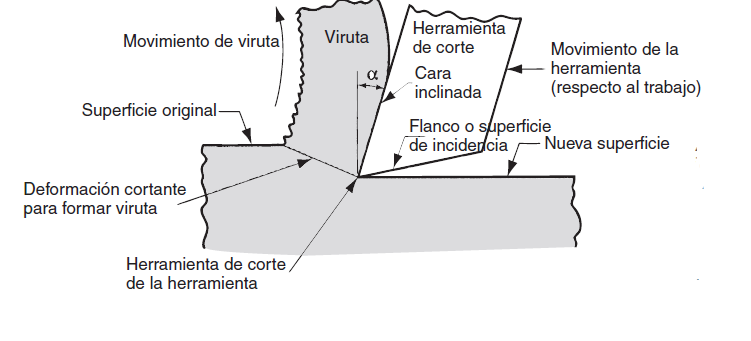
\includegraphics[width = 0.8\textwidth]{Cap1_FormulaciondelProyecto/Figuras/ilustraciondelprocesodemecanizado.PNG}
    \caption{Sección transversal de proceso de maquinado.}
    \citep{groover2007fundamentals}
    \label{ilustraciondelprocesodemecanizado}
\end{figure}


El mecanizada a lo largo de la historia ha sido de los procesos de manufactura el más importante, ya que con el desarrollo de varias de las operaciones de maquinado se puede describir en gran parte la revolución industrial y el crecimiento de las economías basadas en la manufactura. Las siguientes razones exponen la importancia de las operaciones de maquinado desde el punto de vista comercial y tecnológico  \citep{groover2007fundamentals}.\\
\begin{itemize}
\item \textbf{Amplia gama de materiales de trabajo:} El maquinado se puede aplicar a una gran variedad de materiales. Casi todos los metales solidos pueden aplicar a procesos de maquinado, al igual que los compuestos plásticos. Por otro lado, se presentan dificultades al tratar maquinar cerámica por su dureza y fragilidad; no obstante, se puede cortar por medio de maquinado abrasivo\citep{groover2007fundamentals}.

\item\textbf{Variedad de formas y característica geométricas:} El maquina puede ser usado para formar cualquier geometría regular, como superficies planas, agüeros redondos y cilindros. Cuando se introducen variaciones en las trayectorias y forma de las herramientas, se pueden crear formas irregulares, como cuerdas de tornillos y ranuras T.  al implementar en secuencia operaciones de maquinado, se puede producir forma de complejidad y variedad ilimitada\citep{groover2007fundamentals}.

\item\textbf{Precisión dimensional:} El mecanizado puede producir piezas de trabajo con tolerancias muy estrechas de menos de $\pm 0.025$ mm($\pm 0.001$ in). Es más preciso que otros procesos\citep{groover2007fundamentals}.%%te estoy viendo %% EM: hehehehe
\item\textbf{Acabados superficiales de calidad:} Los acabados superficiales con los cuales se puede llegar con el maquinado son mejores que 0.4 micras (16 $\mu$in) \citep{groover2007fundamentals}.
\end{itemize}

Por otra parte, en los procesos de remoción de material existe ciertas desventajas:
\begin{itemize}
    \item \textbf{Desperdicio de material:} El proceso de maquinado es inherentemente un desprecio de materia. En general la viruta generada es la operación es el desprecio. Aunque, por lo general, la viruta generada puede ser reciclada\citep{groover2007fundamentals}.
    \item \textbf{Consumo de tiempo:} El maquinado por lo general toma más tiempo en la formación la pieza que los procesos alternos de formado como el fundido o forjado\citep{groover2007fundamentals}.
\end{itemize}

\section*{Tipos de operaciones de maquinado }

\subsection*{Torneado}

Es la operación de mecanizado se lleva acabo mediante movimientos básicos: el movimiento de corte de material, que es rotativo sobre la pieza, y el movimiento de avance es perpendicular al eje de la rotación y es realizado por la herramienta de corte \citep{Fenoll2009}.\\

\begin{figure}[ht]
    \centering
    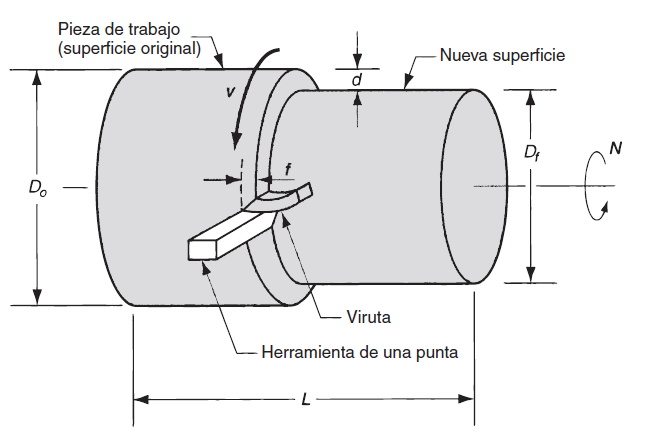
\includegraphics[width = 0.8\textwidth]{Cap1_FormulaciondelProyecto/torneado.PNG}
    \caption{Operación de torneado.}
    \citep{groover2007fundamentals}
    %\label{ilustraciondelprocesodemecanizado}
\end{figure}
\subsubsection*{Parámetros de corte del torneado.}

La velocidad de rotación que usa en el torneado esta relacionada con la velocidad de corte requerida en la superficie cilíndrica de la pieza de trabajo por la siguiente ecuación: 

\begin{equation}
    N=\frac{v}{\pi D_{0}}
\end{equation}
Donde $N$: es la velocidad de rotación que dada en, $Rev./min$; $v$:es la velocidad de corte dada en ,$m/min (ft/min)$; y $D_{0}$ : Es el diámetro original de la pieza y está dado en $m(ft)$.

Cuando en la operación de torneado se quiere reducir el diámetro de trabajo $D_{0}$ al diámetro final $D_{f}$ , el cambio de estos destremina la profundidad de corte $d$: 
\begin{equation}
    D_{f}=D_{0}-2d
\end{equation}
El avance en el torneado por lo general se expresa en $mm/rev (in/rev )$. El avance se puede convertir en velocidad de avance lineal en $mm/min$ mediante la fórmula:
\begin{equation}
    f_{r}=Nf
\end{equation}
 donde $f_{r}$: es velocidad de avance y esta dada en $mm/min (in/min)$; y $f$: es avance y esta en $mm/rev (in/rev).$
 
 El tiempo que toma la operación de torneado de una extremo a otro  a una pieza esta dada por:
 
 \begin{equation}
     T_{m}=\frac{L}{f_{r}}
 \end{equation}
 
 donde $T_{m}$ es el tiempo de maquinado en $min$; y L es la longitud de la pieza cilíndrica en $mm (in)$.
Un cálculo más directo del tiempo de maquinado lo proporciona la ecuación siguiente:
 
 \begin{equation}
     T_{m}=\frac{\pi D_{0} L}{f v}
 \end{equation}
La velocidad volumetrica de Remoción de un materia en $mm^{3}/min(in^{3}/min)$ y se puede determinar más convencionalmente con la siguiente ecuación:
\begin{equation}
    R_{MR}=vfd
\end{equation}

\subsubsection*{Trabajos más usuales realizados en un torno}
El torno normalmente es usado en trabajos de cilindrado, el torneado cónico, el refrentado, el roscado, el taladrado y el maleteado \citep{Fenoll2009}.\\
\begin{itemize}
    \item\textbf{ Cilindrado:} Esta operación permite dar forma uniforme a los diámetros de la pieza cilíndrica mediante desplazamientos de la herramienta de corte paralelamente al eje de giro y el corte perpendicular a este. Con el cilindrado se puede reducir diámetros exteriores y aumentar los diámetros interiores \citep{Fenoll2009} (Figura:\ref{fig:Cilintrado}).
    \item\textbf{Torneado cónico:} Esta operación trabaja con un desplazamiento de la cuchilla no paralela al eje de giro dando piezas con formas cónicas \citep{Fenoll2009}(Figura:\ref{fig:torneadoconico}).
    \item\textbf{Refrentado:} Mediante esta operación se logran planos que son perpendiculares al eje de giro \citep{Fenoll2009}(Figura:\ref{fig:Refretado}).
    \item\textbf{Roscado:} Con el torno se pueden lograr mecanizar rosca, tanto para superficies internas como externas y logra una correcta unión de elementos \citep{Fenoll2009}(Figura:\ref{fig:Roscado}).
    \item\textbf{Taladrado:} Esta operación puede lograrse en el torno con lo broca en el cabezal móvil, y solo se puede hacer en el centro de la pieza \citep{Fenoll2009}(Figura:\ref{fig:Taladrado}).
    \item\textbf{Moleteado:} En este proceso, para dar a la pieza la forma deseada, en lugar de utilizar cuchillas se usan moletas que presionan la pieza mientras gira \citep{Fenoll2009}(Figura:\ref{fig:mo}).
\end{itemize}

\begin{figure}[hbt]
    \centering
    \begin{subfigure}{0.3\textwidth}
        \centering
        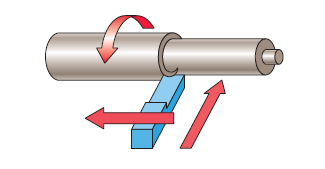
\includegraphics[width=0.9\linewidth]{Cap1_FormulaciondelProyecto/cilindrado.PNG}
        \caption{Cilindrado}
        \label{fig:Cilintrado}
    \end{subfigure} 
    \begin{subfigure}{0.3\textwidth}
        \centering
        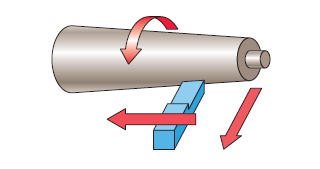
\includegraphics[width=0.9\linewidth]{Cap1_FormulaciondelProyecto/torneadoconico.PNG}
        \caption{Torneado conicó}
        \label{fig:torneadoconico}
    \end{subfigure} 
    \begin{subfigure}{0.3\textwidth}
        \centering
        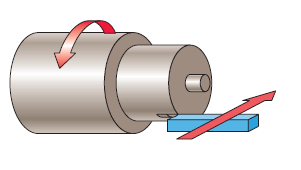
\includegraphics[width=0.9\linewidth]{Cap1_FormulaciondelProyecto/refrentado.PNG}
        \caption{Refrentrado}
        \label{fig:Refretado}
    \end{subfigure}
    \begin{subfigure}{0.3\textwidth}
        \centering
        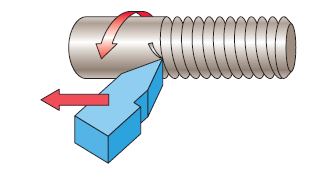
\includegraphics[width=0.9\linewidth]{Cap1_FormulaciondelProyecto/roscado.PNG}
        \caption{Roscado}
        \label{fig:Roscado}
    \end{subfigure}
     \begin{subfigure}{0.3\textwidth}
        \centering
        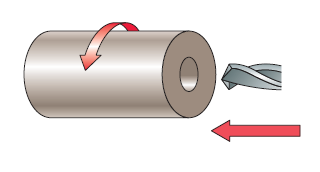
\includegraphics[width=0.9\linewidth]{Cap1_FormulaciondelProyecto/Taladrado.PNG}
        \caption{Taladrado}
        \label{fig:Taladrado}
    \end{subfigure}
     \begin{subfigure}{0.3\textwidth}
        \centering
        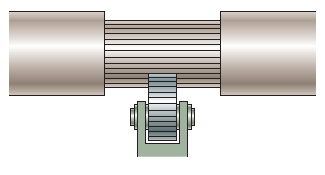
\includegraphics[width=0.9\linewidth]{Cap1_FormulaciondelProyecto/mo.PNG}
        \caption{Moletareado}
        \label{fig:mo}
    \end{subfigure}

    \caption{Trabajos más comunes con Torno}{Fuente: \citep{Fenoll2009}}
    \label{fig:TabajosTorno}
\end{figure}
 

\subsection*{Taladrado}

Es una operación de maquinado donde se una herramienta rotativa cilíndrica que tiene bordes cortantes, dicha herramienta tiene un avance hacia dentro de la pieza de trabajo para formar a un agujero cuyo diámetro es determinado por el diámetro de broca    \citep{groover2007fundamentals}(Figura: \ref{Fig:taradrado}).  

\begin{figure}[ht]
    \centering
    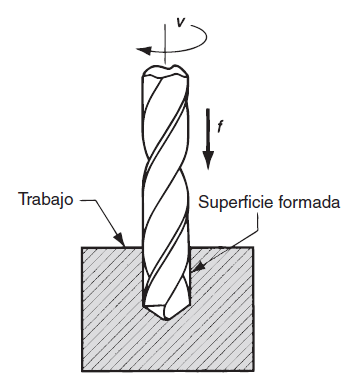
\includegraphics[width = 0.4\textwidth]{Cap1_FormulaciondelProyecto/Figuras/Taradrado1.PNG}
    \caption{Operación de taladrado.}
    \citep{groover2007fundamentals}
    \label{Fig:taradrado}
\end{figure}

\subsubsection{Parámetros de corte en el taladrado}

En la operación de taladrado la velocidad de corte es la velocidad en la superficie del diámetro exterior de la herramienta de corte. Este parámetro se especifica así por conveniencia, sin embargo, casi toda la operación de corte se realiza a velocidad mas bajas cercanas al eje de rotación. Para fijar una velocidad de corte requerida en el taladrado, se necesita determinar la velocidad de giro de la broca por su diámetro. Si $N$ representa las $rev/min$ del, entonces \citep{groover2007fundamentals}:

\begin{equation}
    N=\frac{v}{\pi D}
\end{equation}

Donde v es la velocidad de corte ($in/mm$), el diámetro de la broca es $D$, mm(in). En el taladrado alguna operación la superficie de la pieza de trabajo gira sobre la herramienta, pero la fórmula se aplica igual\citep{groover2007fundamentals}.

En la operación de taladrado, el avance $f$ esta dado en $mm/rev(in/rev)$. Lo que se recomienda es que la velocidades sean aproximadamente proporcionales al diámetro de la broca. Generalmente los avances altos se dan con brocas con diámetros grandes. El avance se puede convertir en velocidad de avance si se usa la misma ecuación de torneado\citep{groover2007fundamentals}:

\begin{equation}
    f_{r}=N n_{t} f
\end{equation}
 
\begin{figure}[hbt]
    \centering
    \begin{subfigure}{0.3\textwidth}
        \centering
        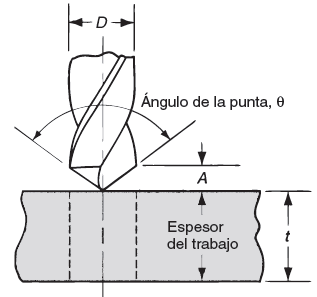
\includegraphics[width=0.9\linewidth]{Cap1_FormulaciondelProyecto/Figuras/taladradopasante.PNG}
        \caption{Agujero pasante}
        \label{fig:AgujeroPasado}
    \end{subfigure} 
     \begin{subfigure}{0.3\textwidth}
        \centering
        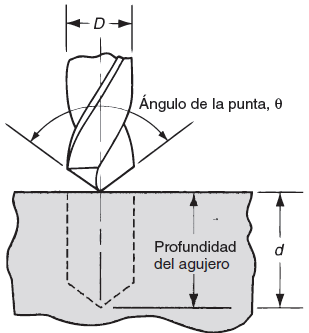
\includegraphics[width=0.9\linewidth]{Cap1_FormulaciondelProyecto/Figuras/taladradociego.PNG}
        \caption{Agujero ciego}
        \label{fig:AgujeroCiego}
    \end{subfigure} 
    
    \caption{Tipos de agujeros en el taladrados}{Fuente: \citep{groover2007fundamentals}}
    \label{fig:TiposDeAngujeros}
\end{figure}

Donde $f_{r}$ es la velocidad de avance en $mm/min (in/min).$
La operación de taladrado puede hacer dos tipos de aguajero; aguajeros ciegos (Figura:\ref{fig:AgujeroCiego}) y agujeros completos (Figura:\ref{fig:AgujeroPasado}). En los agujeros completos o pasados, la broca atraviesa la pieza de trabajo; en los aguajeros ciego no es así.  Para determinar el tiempo requerido para hacer un agujero pasado se usa la siguiente fórmula\citep{groover2007fundamentals}:

\begin{equation}
    T_{m}=\frac{t+A}{f_{r}}
\end{equation}
Donde $T_{m}$ es el tiempo de maquinado (taladrado) expresado en minutos(min), con un espesor en la pieza de trabajo $t$ en $mm(in)$, una velocidad de avance $f_{r}$ en $mm/min(in/min)$ y $A$ es la tolerancia de aproximación la cual tiene en consideración el ángulo de la punta de la broca, esta tolerancia esta se halla de la siguiente forma\citep{groover2007fundamentals}:
\begin{equation}
A=0.5*D*tan(90-\frac{\theta}{2})    
\end{equation}
Donde $A$ es la tolerancia de aproximación en $mm(in)$ y $theta$ es el ángulo de la punta de la broca.   
    
Por otro lado, en un agujero ciego la profundidad $d$ esta definida como la distancia entre la superficie de la pieza de trabajo y la punta del agujero como se ve en la Figura:\ref{fig:AgujeroCiego}. En este caso por la definición anterior el ángulo no afecta en el tiempo de maquinado. Por ende, el tiempo de maquinado este dado por lo siguiente:

\begin{equation}
    T_{m}=\frac{d}{f_{r}}
\end{equation}

La velocidad de remoción de materia en el taladrado se puede obtener con el producto entre sección trasversal de la broca y la velocidad de avance. La siguiente ecuación solo es validad después que la broca alcance el diámetro completo y no incluye la aproximación de la broca a la pieza de trabajo\citep{groover2007fundamentals}:
\begin{equation}
    R_{MR}=\frac{\pi D^{2} f_{r}}{4}
\end{equation}

\subsection*{Fresado} La operación de fresado consiste en corte la superficie de la una pieza con una herramienta rotativa, que esta provista de múltiples aristas cortantes que se encuentra ubicadas simétricamente alrededor del eje gira \citep{Fenoll2009}.

Hay dos operaciones básicas de fresado, fresado periférico (\ref{fig:FP}) y fresado Frontal(\ref{fig:FF}.

\begin{figure}[hbt]
    \centering
    \begin{subfigure}{0.4\textwidth}
        \centering
        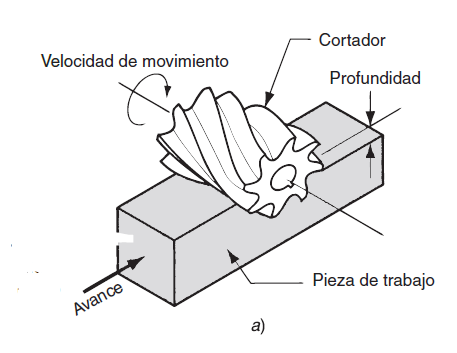
\includegraphics[width=0.9\linewidth]{Cap1_FormulaciondelProyecto/FresadoPeriferico.PNG}
        \caption{Fresado periférico}
        \label{fig:FP}
    \end{subfigure} 
 \begin{subfigure}{0.4\textwidth}
        \centering
        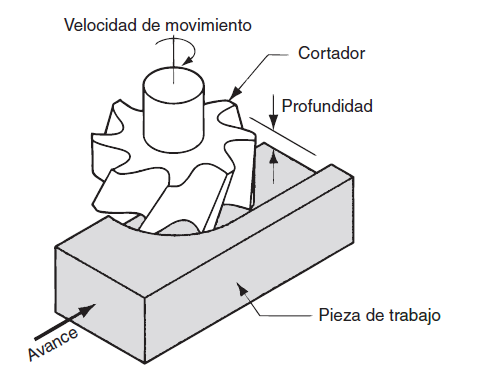
\includegraphics[width=0.9\linewidth]{Cap1_FormulaciondelProyecto/FresadoFrontal.PNG}
        \caption{Fresado Frontal}
        \label{fig:FF}
    \end{subfigure} 
    \caption{Operaciones basicas de fresado}{Fuente: \citep{groover2007fundamentals}}
    \label{fig:FresadoBasico}
\end{figure}

\subsubsection*{Fresado periférico}
El fresado periférico o también llamado fresado plano trabaja con el eje de la herramienta paralelo a la superficie de la pieza que se esta maquinando como se ve en la figura \ref{fig:FP}. La operación se realiza por la periferia exterior del cortador.

El fresado periférico se puede clasificar en varios tipos como:
\begin{itemize}
    \item \textbf{Fresado de placa:} Esta es la operación básica del fresado periférico donde el ancho de la fresa se extiende más allá de la pieza de trabajo en ambos extremos(figura\ref{fig:Fresadodeplaca}). 
    \item \textbf{Fresado de Ranurado:} Esta operación el anche de la fresa es menor que el ancho de la pieza de trabajo, esto produce una ranura en la pieza. Cuando la fresa es muy delgada esta operación se pude usas para tallar ranuras angostas o corta una pieza en dos, esta ultima variante se conoce como fresado aserrado (figura\ref{fig:Fresadoderanurado}). 
    \item \textbf{Fresado lateral:} Esta operación es la cual, la fresa el lado de una pieza (figura\ref{fig:Fresadolateral}). 
    \item \textbf{Fresado paralelo simultaneo:} Esta operación en esencia es el mismo fresado natural con la diferencia que, el corte realizado es en ambos lados de la pieza de trabajo(figura\ref{fig:Fresadosimultaneo}).  
\end{itemize}
\begin{figure}[hbt]
    \centering
    \begin{subfigure}{0.4\textwidth}
        \centering
        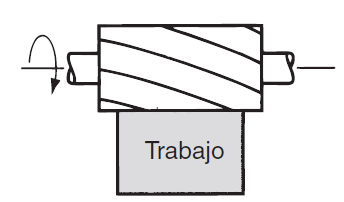
\includegraphics[width=0.9\linewidth]{Cap1_FormulaciondelProyecto/Figuras/FrsadodePlaca.PNG}
        \caption{Fresado de placa}
        \label{fig:Fresadodeplaca}
    \end{subfigure} 
    \begin{subfigure}{0.4\textwidth}
        \centering
        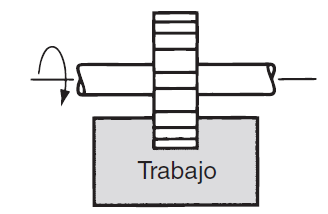
\includegraphics[width=0.9\linewidth]{Cap1_FormulaciondelProyecto/Figuras/FrsadodeRanurado.PNG}
        \caption{Fresado de Ranurado}
        \label{fig:Fresadoderanurado}
    \end{subfigure} 
    \begin{subfigure}{0.4\textwidth}
        \centering
        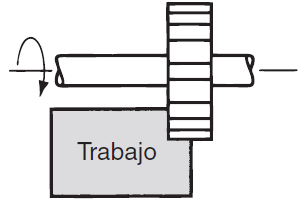
\includegraphics[width=0.9\linewidth]{Cap1_FormulaciondelProyecto/Figuras/Fresadolateral.PNG}
        \caption{Fresado lateral}
        \label{fig:Fresadolateral}
    \end{subfigure}
    \begin{subfigure}{0.4\textwidth}
        \centering
        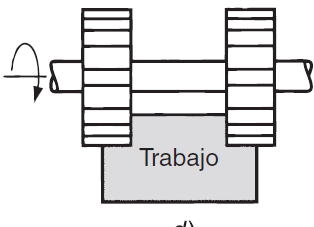
\includegraphics[width=0.9\linewidth]{Cap1_FormulaciondelProyecto/Figuras/FresadoSimuntaneo.PNG}
        \caption{Fresado simultaneo}
        \label{fig:Fresadosimultaneo}
    \end{subfigure}
    
    \caption{Operaciones de fresado periférico}{Fuente: \citep{groover2007fundamentals}}
    \label{fig:FresadoPeriferico}
\end{figure}

La operación fresado periférico tienes dos direcciones de rotación para realizar los cortes. Estas direcciones son conocidas como fresado convencional o ascendente y fresado descendente.
La dirección ascendente, la dirección del movimiento de los dientes es opuesto a la dirección de avance como se muestra en figura\ref{fig:Fresadoascendente}. En el fresado ascendente, la viruta por cada diente de cortador comienza siendo muy delgada y aumenta su espesor con el paso del diente. Por otro lado, el fresado descendente la dirección del movimiento va a favor de la dirección del avance. la viruta empieza gruesa y se va reduciendo con el paso del diente \citep{groover2007fundamentals} (figura\ref{fig:Fresadodescendente}).  

La dirección de la fuerza es tangencial a la periferia de la herramienta de corte. En el fresado ascendente tiende a levantar la pieza ya que al salir los dientes salen de la pieza de trabajo. En el fresado descendente, la dirección de la fuerza de corte es hacia debajo, por esa razón la pieza de trabajo se mantiene conta la base de la máquina de fresado \citep{groover2007fundamentals}. 
\begin{figure}[hbt]
    \centering
    \begin{subfigure}{0.4\textwidth}
        \centering
        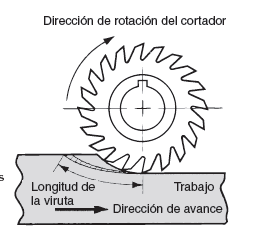
\includegraphics[width=0.9\linewidth]{Cap1_FormulaciondelProyecto/Figuras/fresadoascendente.PNG}
        \caption{Fresado ascendente}
        \label{fig:Fresadoascendente}
    \end{subfigure} 
    \begin{subfigure}{0.4\textwidth}
        \centering  
        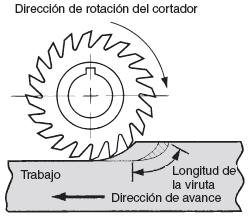
\includegraphics[width=0.9\linewidth]{Cap1_FormulaciondelProyecto/Figuras/fresadodescendente.PNG}
        \caption{Fresado descendente}
        \label{fig:Fresadodescendente}
    \end{subfigure}
    
    \caption{Dos formas de fresado}{Fuente: \citep{groover2007fundamentals}}
    \label{fig:formaFresadoperiferico}
\end{figure}
\subsubsection*{Fresado frontal}
 La característica del Fresado frontal que el eje de la fresa es perpendicular a la superficie de trabajo y el mecanizado de realiza tanto en las orillas, como en el extremo y fuero de la periferia de la fresa. Como en el fresado de periferia, el fresado frontal tiene diversas formas como (figura \ref{fig:FresadoFrontal}):
 
\begin{figure}[hbt]
    \centering
    \begin{subfigure}{0.25\textwidth}
        \centering
        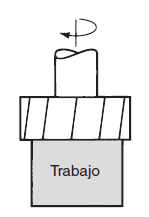
\includegraphics[width=0.9\linewidth]{Cap1_FormulaciondelProyecto/Figuras/a.PNG}
        \caption{Fresado frontal convencional}
        \label{fig:FresadoFC}
    \end{subfigure} 
    \begin{subfigure}{0.25\textwidth}
        \centering
        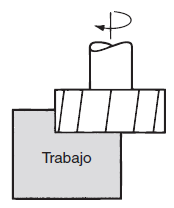
\includegraphics[width=0.9\linewidth]{Cap1_FormulaciondelProyecto/Figuras/b.PNG}
        \caption{Fresado frontal parcial}
        \label{fig:FresadoFP}
    \end{subfigure}
    \begin{subfigure}{0.25\textwidth}
        \centering
        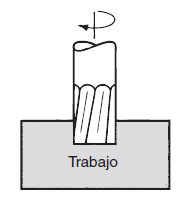
\includegraphics[width=0.9\linewidth]{Cap1_FormulaciondelProyecto/Figuras/c.PNG}
        \caption{Fresado terminal}
        \label{fig:FresadoT}
    \end{subfigure}
    \begin{subfigure}{0.25\textwidth}
        \centering
        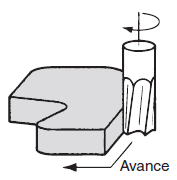
\includegraphics[width=0.9\linewidth]{Cap1_FormulaciondelProyecto/Figuras/d.PNG}
        \caption{Fresado de perfiles}
        \label{fig:Fresadodeperfiles}
    \end{subfigure}
    \begin{subfigure}{0.25\textwidth}
        \centering
        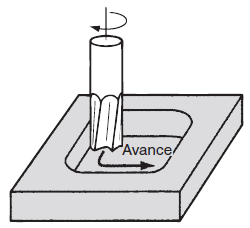
\includegraphics[width=0.9\linewidth]{Cap1_FormulaciondelProyecto/Figuras/e.PNG}
        \caption{Fresado de cavidades}
        \label{fig:Fresadodecavidades}
    \end{subfigure}
    \begin{subfigure}{0.25\textwidth}
        \centering
        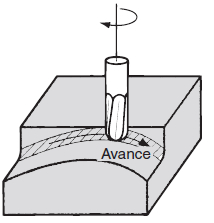
\includegraphics[width=0.9\linewidth]{Cap1_FormulaciondelProyecto/Figuras/f.PNG}
        \caption{Fresado de contorno superficial}
        \label{fig:FresadoCs}
    \end{subfigure}
    \caption{Fresado Frontal}{Fuente: \citep{groover2007fundamentals}}
    \label{fig:FresadoFrontal}
\end{figure} 


\begin{itemize}
    \item \textbf{Fresado frontal convencional:} En esta operación el diámetro de la fresa es mas grande que el ancha de pieza a trabajar, de tal modo que la fresa sobre pasa la pieza en ambos extremos(figura\ref{fig:FresadoFC}).
    \item\textbf{Fresado frontal parcial:} En esta operación la fresa solo sobrepasa una de los extremos de la pieza(figura\ref{fig:FresadoFP}).
    \item\textbf{Fresado terminal:} En esta operación el diámetro es menor que el ancho de la pieza de trabajo, formando una ranura dentro de la pieza(figura\ref{fig:FresadoT}).
    \item\textbf{Fresado de perfiles:} Esta operación es similar a l fresado terminal, con la diferencia que se corta una pieza plana en la periferia(figura\ref{fig:Fresadodeperfiles}).
    \item\textbf{Fresado de cavidades:} Esta operación es también similar al fresado terminal que se usa para fresar cavidades en superficies planas(figura\ref{fig:Fresadodecavidades}).
    \item\textbf{Fresado de contorno superficial:} En esta operación una fresa con punta de bola se coloca a avanzar hacia delante y hacia atrás, y hacia un lado y otro del trabajo, a lo largo de una trayectoria curvilínea a pequeños intervalos para crear una superficie tridimensional(figura\ref{fig:FresadoCs}). 
    
\end{itemize} 

\subsubsection*{Parámetros de corte del fresado}
La velocidad de corte se determina con el diámetro exterior de la fresa. Esta velocidad de corte se puede convertir en velocidad de rotación del husillo con la siguiente formula:
\begin{equation}
    N=\frac{v}{\pi D}
\end{equation}

El avance del fresado por lo general se determina como el avance por diente cortante o también llamado \textbf{carga de viruta}, este representa el tamaño de la viruta. Esto se puede traducir a velocidad de avance, considerando la velocidad del husillo y el número de diente de la fresa, como en lo siguiente \citep{groover2007fundamentals}:
\begin{equation}
    f_{r}=N n_{t} f
\end{equation}

Donde $f_{r}$ es la velocidad de avance en $mm/min (in/min)$ , $N$ es la velocidad del husillo en $rev/diente$, $n_{t}$  es el numero de dietes de la fresa y el $f$ es la carga de viruta en $mm/diente(in/dientes)$. 

En el fresado la remoción de materia se determina con el producto de la velocidad de avance con el área transversal del corte. Siendo así, si una operación de fresado corta una pieza la velocidad de remoción estar dada por el ancho $w$, la profundidad $d$ y la ecuación es \citep{groover2007fundamentals}:
\begin{equation}
    R_{MR}=w d f_{r}
\end{equation}
Este cálculo ignora la entrada inicial de la fresa antes de su enganche por completo. Aplicar la ecuación enterior es conveniente en los fresados terminales, lateral, frontal y otras operaciones, haciendo ajustes al cálculo del área transversal de la sección recta del corte \citep{groover2007fundamentals}.

\begin{figure}[hbt]
        \centering
        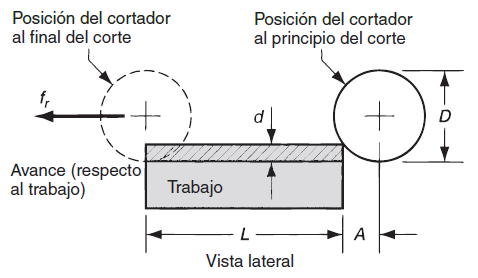
\includegraphics[width=0.6\linewidth]{Cap1_FormulaciondelProyecto/Figuras/fresadaPentrada.PNG}
    \caption{Fresado periferico que muestra la entrada de la fresa}{Fuente: \citep{groover2007fundamentals}}
    \label{fig:fresadaPentrada}
\end{figure}

El tiempo que requiere la operación de fresado en una pieza de trabajo con una longitud $L$ debe tomar en consideración la longitud de aproximación requerida para engancha la pieza completamente. Si se considera el caso del fresado periférico que se observa en la figura \ref{fig:fresadaPentrada}, para determinar el tiempo de la operación de fresado en la placa, la distancia de aproximación $A$ para alcanzar la velocidad de corte se determina mediante la siguiente formula \citep{groover2007fundamentals}:

\begin{equation}
    A=\sqrt{d(D-d)}
\end{equation}
Donde $d$ es la profundidad de corte en mm(in) y $D$ es el diámetro de la fresa. Por lo tanto, el cálculo de tiempo de fresado $T_{m}$ es:
\begin{equation}
    T_{m}=\frac{L+A}{f_{r}}
\end{equation}

\begin{figure}[hbt]
    \centering
    \begin{subfigure}{0.5\textwidth}
        \centering
        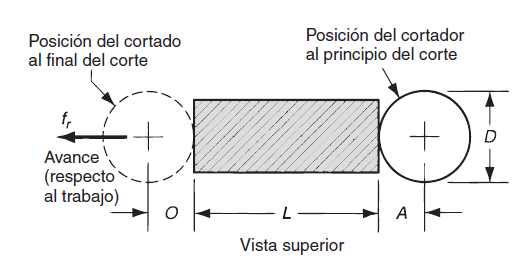
\includegraphics[width=0.9\linewidth]{Cap1_FormulaciondelProyecto/Figuras/fresadoFCP.PNG}
        \caption{Fresador centrado en la pieza de trabajo}
        \label{fig:fresadoFCP}
    \end{subfigure} 
    \begin{subfigure}{0.4\textwidth}
        \centering  
        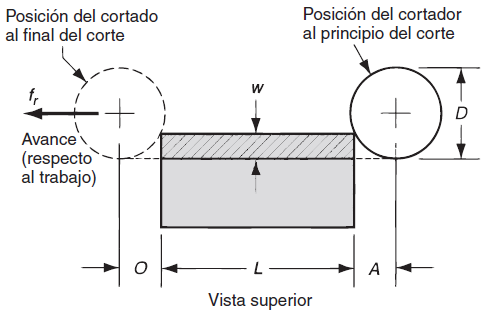
\includegraphics[width=0.9\linewidth]{Cap1_FormulaciondelProyecto/Figuras/FresadodesplasaL.PNG}
        \caption{Cortador con desplazamiento hacia un lado del trabajo}
        \label{fig:FresadodesplasaL}
    \end{subfigure}
    
    \caption{Distancias de aproximación y recorrido adicional}{Fuente: \citep{groover2007fundamentals}}
    \label{fig:distanciasyrecoridoincial}
\end{figure}

Para el fresado frontal hay dos casos posibles para lo cuales se acostumbra dejar, aparte de una distancia de aproximación $A$ una distancia $O$. En los dos casos la distancia $A=O$. En primer caso es cuando la fresa se centra sobre la pieza de trabajo rectangular (figura\ref{fig:fresadoFCP}). En este caso $A$ y $O$ son iguales a la mitad del diámetro.
\begin{equation}
    A=O=\frac{D}{2}
\end{equation}
Para el caso dos (figura\ref{fig:FresadodesplasaL}) donde sobresale uno de los lados del trabajo, las distancias de aproximación y la adicional en tanta dadas por:
Donde $w$ es el ancho de corte en mm(in). Por lo tanto, el tiempo de fresado por este dado por:

\begin{equation}
    T_{m}=\frac{L+2A}{f_{r}}
\end{equation}

Los parámetros de velocidad de corte y profundidad dependen de la vida útil de la herramienta. Para ser conservadores estos valores se toman de algunos fabricantes de la herramienta de corte. Los valores tienen en cuenta el material de la pieza de trabajo y el tipo de operación. Ejemplo de esto se observa en la tabla \ref{table:Parametrosdefresado}, en donde se muestra los parametros de corte para fresado de para acero endurecido (45- 55 HRC).

\begin{center}
    \begin{longtable}{>{\columncolor[gray]{0.90}} p{0.15\textwidth} p{0.15\textwidth} p{0.15\textwidth} p{0.15\textwidth} p{0.25\textwidth}}
    \rowcolor[gray]{0.85}
    \textbf{Diametro de la fresa} & \textbf{Revoluciones}  & \textbf{Avance}  & \textbf{Profundidad radial} & \textbf{Profundidad axial} \\
    \rowcolor[gray]{0.85} (mm) & (RPM) & (mm/min) & & \\ \hline \endhead
        {2} & 8000&120 &0.05D &1D para escuadra \\
            &     &    &      &0.05D para ranurado\\ \hline
        {3} & 5000&120 &0.05D &1D para escuadra\\
            &     &    &      &0.1D para ranurado\\ \hline
        {4} & 4000&120 &0.05D &1D para escuadra\\
            &     &    &      &0.1D para ranurado\\ \hline
        {5} & 3200&120 &0.05D &1D para escuadra\\
            &     &    &      &0.1D para ranurado\\ \hline 
        {6} & 2700&120 &0.05D &1D para escuadra\\
            &     &    &      &0.1D para ranurado\\ \hline
        {8} & 2000&110 &0.05D &1D para escuadra\\
            &     &    &      &0.1D para ranurado \\ \hline
        {10}& 1600&100 &0.05D &1D para escuadra\\
            &     &    &      &0.1D para ranurado\\ \hline 
        {12}& 1300&100 &0.05D &1D para escuadra\\
            &     &    &      &0.1D para ranurado\\ \hline
        \caption{Parametros de corte para fresado} {Fuente:\citep{catalogue:CatalogoC005s}}
        \label{table:Parametrosdefresado}
    \end{longtable}
\end{center}

\subsection{Fundamentos de la Robotica}

%\subsection*{Manipuladores Seriales}
%
%\subsection*{Manipuladores Paralelos}
%Los manipuladores paralelos, también conocidos como robots paralelos, %son familia de mecanismos, caracterizados por presentar dos %plataformas, una fija (base) y otra móvil (plataforma), conectadas %por, al menos dos, cadenas cinemáticas independientes, ya sean %abiertas o cerradas. Según los grados de libertad del dispositivo es %igualmente requerido número de cadenas cinemáticas, debido a que cada %una es accionada por un actuador. Estos actuadores pueden ser %ubicados cerca de la base, lo cual permite que no sea parte de las %cargas inerciales del mecanismo y su potencia sea utilizada más %ampliamente en el movimiento del dispositivo. %Para comprender más %sobre los robots paralelos, en las próximas secciones se explicará un %poco de su historia, la manera de analizar su cinemática y un método %para el análisis dinámico.
%
%\begin{figure}[t]
%    \centering
%    \begin{subfigure}{0.4\textwidth}
%        \centering
%        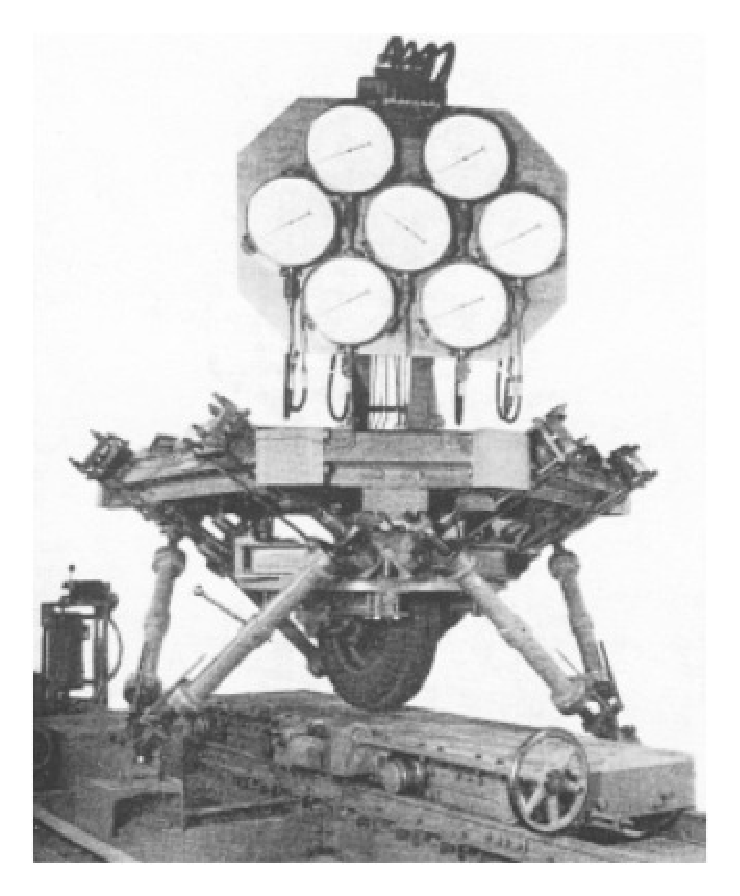
\includegraphics[width=0.8\linewidth]{Cap1_FormulaciondelProy%ecto/Figuras/GoughPlatform.pdf}
%        \caption{Plataforma de Gough}
%        \label{fig:GoughPlatform}
%    \end{subfigure} 
%    \begin{subfigure}{0.4\textwidth}
%        \centering
%        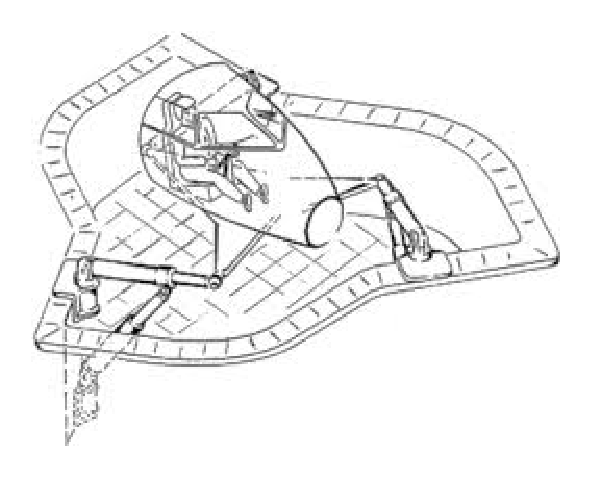
\includegraphics[width=0.8\linewidth]{Cap1_FormulaciondelProy%ecto/Figuras/StewartPlatform.pdf}
%        \caption{Plataforma de Stewart}
%        \label{fig:StewartPlatform}
%    \end{subfigure}
%    \begin{subfigure}{0.8\textwidth}
%        \centering
%        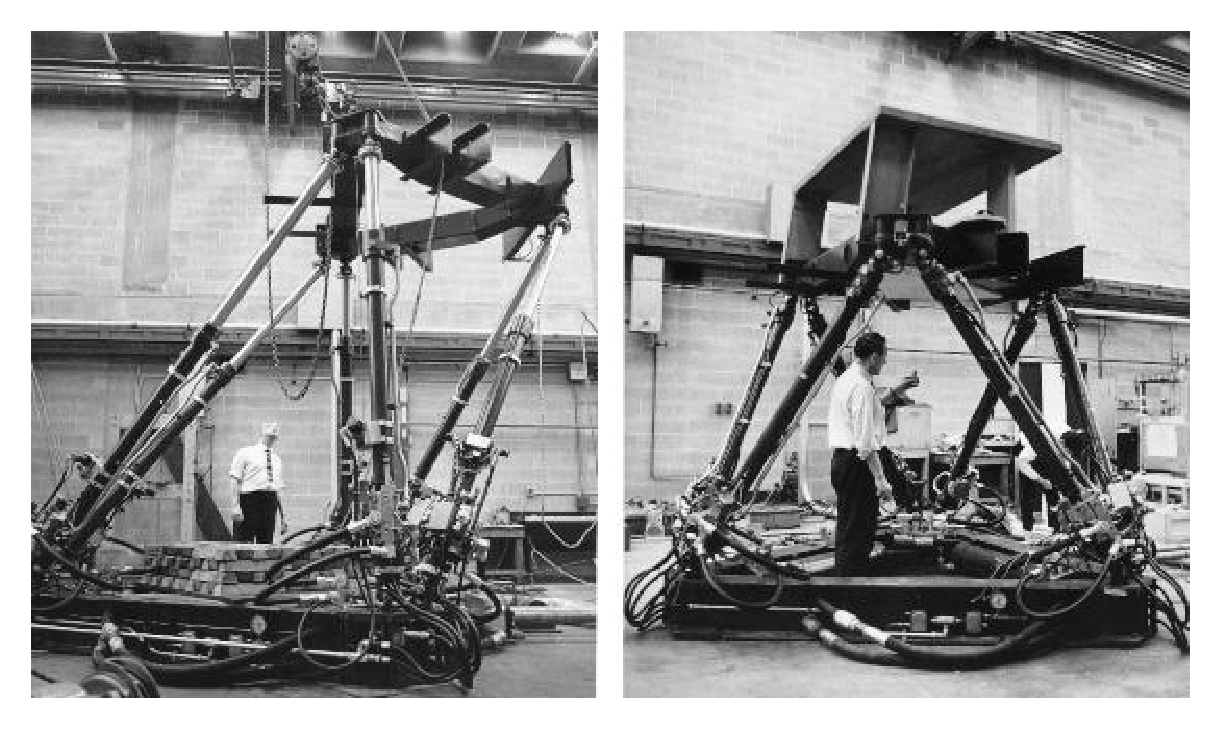
\includegraphics[width=0.5\linewidth]{Cap1_FormulaciondelProy%ecto/Figuras/KlausCappelSimulators.pdf}
%        \caption{Plataforma de Stewart}
%        \label{fig:KlausCappelSimulators}
%    \end{subfigure}
%    \caption{Mecanismos Octaedro Hexápodo}{Fuente: %\citep{zhang2009parallel}}
%    \label{fig:MechanismPriors}
%\end{figure}

\subsection*{Criterio de Diseño y Movilidad}

Los grados de libertad (GDL) de un mecanismo representa la cantidad de movimientos independientes que pueden desarrollar el mecanismo. Otra interpretación es el número de entradas independientes que requeridos para satisfacer completamente de la configuración del dispositivo. Para determinar los grados de libertad de un mecanismo es utilizado el criterio de Chebyshev–Grübler–Kutzbach \citep{taghirad2013parallel}, ver ecuación \ref{Eq:ChebyshevCriterion}. Este criterio hace una relación del número de eslabones del mecanismo, incluyen la base, además del número y tipo de juntas, con los grados de libertad del mecanismo; por otra parte, para esta relación se define los grados de libertad de movimiento permitidos en este espacio, siendo $\lambda = 3$ para mecanismos planos y $\lambda = 6$ para un mecanismo general en el espacio.

\begin{equation}
    F = \lambda \left( n - j - 1 \right) + \sum_{i=1}^j f_i
    \label{Eq:ChebyshevCriterion}
\end{equation}

donde:
\begin{itemize}
    \item $F$ : Grados de libertad del mecanismo
    \item $\lambda$ : Grados de libertad del espacio
    \item $n$ : número de eslabones en el mecanismo, incluyendo la base
    \item $j$ : número de juntas binarias en el mecanismo
    \item $f_i$ : grados de movimiento relativo permitidos por la $i$-esima junta.
\end{itemize}

\subsection*{Cinemática}
La cinemática relaciona el movimiento de los cuerpos sin considerar las fuerzas y momentos que lo generan, siendo una herramienta fundamental para el diseño del robot, análisis, control y simulación. Por lo tanto, la comunidad académica ha centrado en aplicar eficientemente representaciones de las posiciones y orientaciones, como sus derivadas con respecto al tiempo, para resolver los problemas fundamentales de la cinemática \citep{waldron2016kinematics}.

\subsubsection*{Posiciones y Traslaciones} 
La posición de un elemento relativo $i$ a un sistema coordenado $A$ es denotado por un vector,$~^{A}\vec{P}_i$, de 3 componentes, en una columna, las cuales son las respectivas proyecciones del vector sobre los ejes coordenados. Del mismo modo, el vector puede ser representado por coordenadas cilíndricas o esféricas, las cuales tienen ventajas en el análisis de mecanismo en donde se incluyen juntas esféricas o revolutas \citep{waldron2016kinematics}.

\begin{equation}
    ~^{A}\vec{P}_i = \left[\begin{array}{c} ~^{A}P_{ix} \\ ~^{A}P_{iy} \\ ~^{A}P_{iz} \end{array}\right]
\end{equation}

Una traslación es un desplazamiento en donde ningún punto en el cuerpo rígido permanece en su posición inicial y todas las líneas rectas del cuerpo rígido mantienen paralelas a su orientación original.

\subsubsection*{Orientación y Rotación}
Una rotación es un desplazamiento en donde al menos un punto en el cuerpo rígido permanece en la posición inicial y no todas las líneas en el cuerpo permanece paralelo a la orientación inicial \citep{waldron2016kinematics}. Un método conveniente de describir las rotaciones es por medio de las matrices de rotación, una matriz 3x3 que muestra el movimiento del sistema coordenado $B$ con respecto al sistema coordenado $A$ \citep{taghirad2013parallel}.

\begin{equation}
    ^{A}R_{B} = \left[ \begin{array}{ccc}
        r_{11} & r_{12} & r_{13}  \\
        r_{21} & r_{22} & r_{23}  \\
        r_{31} & r_{32} & r_{33}
    \end{array} \right]
\end{equation}

Considerando la rotación solo es a lo largo de uno de los ejes cartesianos, la matrices obtenidas serían las siguientes:

\begin{subequations}
    \begin{eqnarray}
        ^{A}R_{B} = R_x \left( \alpha \right) = \left[ \begin{array}{ccc} 1 & 0 & 0  \\ 0 & \cos\left(\alpha\right)  & -\sin\left(\alpha\right)  \\ 0 & \sin\left(\alpha\right) & \cos\left(\alpha\right) \end{array} \right] \\
        ^{A}R_{B} = R_y \left( \alpha \right) = \left[ \begin{array}{ccc} \cos\left(\alpha\right) & 0 & \sin\left(\alpha\right)  \\ 0 & 1 & 0  \\ -\sin\left(\alpha\right) & 0 & \cos\left(\alpha\right) \end{array} \right] \\
        ^{A}R_{B} = R_z \left( \alpha \right) = \left[ \begin{array}{ccc} \cos\left(\alpha\right) & -\sin\left(\alpha\right) & 0  \\ \sin\left(\alpha\right) & \cos\left(\alpha\right) & 0  \\ 0 & 0 & 1 \end{array} \right]
    \end{eqnarray}
\end{subequations}
%\subsection{Método de Optimización Heurístico}
%\subsection{Método de Elementos Finitos}